\documentclass[12pt,a4paper]{article}
\usepackage[utf8]{inputenc}
\usepackage[russian]{babel}
\usepackage[OT1]{fontenc}
\usepackage{mathtools}
\usepackage{amsfonts}
\usepackage{amssymb}
\usepackage{enumitem}
\usepackage{alltt}
\usepackage{graphicx}
\usepackage{indentfirst}
\usepackage{caption}
\usepackage{float}
\usepackage{wrapfig}
\setlength{\parindent}{0.75cm}
\graphicspath{{pictures/}}
\DeclareGraphicsExtensions{.png}
\usepackage[left=15mm,right=15mm,top=2cm,bottom=2cm]{geometry}
\author{Глотов Алексей}
\begin{document}
\newpage
\begin{center}
\footnotesize{{ГОСУДАРСТВЕННОЕ АВТОНОМНОЕ ОБРАЗОВАТЕЛЬНОЕ УЧРЕЖДЕНИЕ}\break
{ВЫСШЕГО ОБРАЗОВАНИЯ}
\break
{\bf {МОСКОВСКИЙ ФИЗИКО-ТЕХНИЧЕСКИЙ ИНСТИТУТ}}
\break
\small{(НАЦИОНАЛЬНЫЙ ИССЛЕДОВАТЕЛЬСКИЙ УНИВЕРСИТЕТ)}}
\break
\hfill \break
\hfill \break
\begin{center}
\normalsize{Кафедра общей физики}
\end{center}
\hfill \break
\hfill \break
\hfill \break
\hfill \break

\begin{center}
\normalsize {Вопрос по выбору}
\end{center}
\hfill \break\\
\large{Рассмотрение работы автоколебательной системы на примере храпового маятника}
\end{center}
\hfill \break
\hfill \break
\hfill \break
\hfill \break
\hfill \break
\hfill \break
\hfill \break
\hfill \break
\hfill \break
\hfill \break
\begin{flushright}
Обучающийся: Глотов А.А
\end{flushright}
\hfill \break
\hfill \break
\hfill \break
\hfill \break
\hfill \break
\hfill \break
\hfill \break
\hfill \break
\hfill \break
\hfill \break
\hfill \break
\hfill \break
\hfill \break
\begin{center}
Долгопрудный \break
 2022
\end{center}
\thispagestyle{empty}
\newpage
\par Автоколебаниями называются незатухающие колебания в диссипативной (открытой) системе, поддерживаемые за счёт внешнего источника, но, в отличие от вынужденных колебаний, при отсутствии переменного внешнего воздействия: период и амплитуда определяются свойствами самой системы таким образом, что потери энергии в точности компенсируются поступлением энергии извне. Примерами автоколебательных систем могут служить:
\begin{itemize}
\item Незатухающие колебания маятника часов за счёт постоянного действия силы тяжести заводной гири
\item Колебания скрипичной струны под действием равномерно движущегося смычка
\item Звучание органной трубы при постоянной скорости подачи воздуха (стоячая волна)
\item  Колебания листьев деревьев под действием равномерного потока воздуха
\item Работа поршневых паровых двигателей и двигателей внутреннего сгорания
\item Маятник Фруда
\end{itemize}
Любая автоколебательная система состоит из 4 частей:
\begin{itemize}
\item Колебательная система
\item Источник энергии, компенсирующий потери энергии
\item "Клапан" - устройство (или часть структуры автоколебательной системы), регулирующее поступление энергии в колебательную системы 
\item Устройство (или часть структуры автоколебательной системы) "обратной связи", управляющее работой "клапана" за счет процессов самой колебательной системы
\end{itemize}
Иначе говоря, поступление энергии извне в колебательную системы зависит только от ее текущего состояния
\par Изучим принцип действия маятниковых часов подробнее, рассмотрев 4 модели. При этом (сейчас и в дальнейшем) выполняются следующие условия: удар происходит ровно один раз за период, система полностью циклична, то есть на временном промежутке, равному периоду, система находится в точности одинаковом состоянии.  \hfill \break
\begin{figure}[H]
\centering
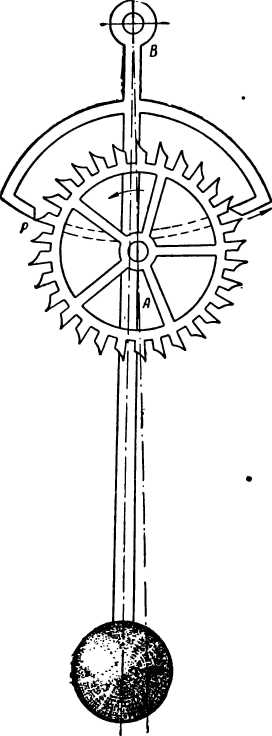
\includegraphics[width=6cm, height=12cm]{ВПВ_5}
\caption{Храповый маятник}
\label{pic:1}
\end{figure}
1) Случай линейного трения, т.е. зависимость силы трения от скорости.  \hfill \break
d - логарифмический декремент (малого) затухания \hfill \break
$\Delta{u}$ - приращение скорости системы, получаемое при ударе
\begin{equation}
\text{непосредственно перед ударом} \;\;\;\; u^{'}=u_{1}e^{-d}
\end{equation}
\begin{equation}
\text{сразу после удара} \;\;\;\; u_{2}=u_{1}e^{-d} + \Delta{u}
\end{equation}
Необходимое условие цикличности процесса: $u_{1}=u_{2}=u$, где u - стационарная амплитуда скорости. Тогда
\begin{equation}
u=\frac{\Delta{u}}{1-e^{-d}}
\end{equation}
\begin{figure}[H]
\centering
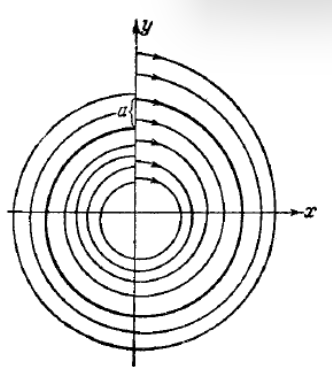
\includegraphics[width=6cm, height=6cm]{ВПВ_1}
\caption{Фазовый портрет колебаний}
\label{pic:1}
\end{figure}
Таким образом, независимо от начального толчка, будут совершаться циклические колебания. Это лишь частично соответствует реальности, т.к. в настоящей модели требуется придать изначальный толчок конечной величины для того чтобы часы пошли \hfill \break
1.2)Рассмотрим немного более "реалистичную ситуацию": $u^{2}_{2}-u^{2}_{1}=k^{2}=const$, т.к. при одинаковом повороте зубчатого колеса, на одну величину смещается и груз, то есть совершает конечную одинаковую работу. Тогда ур-ие (1) неизменно, второе примет вид 
\begin{equation}
u_{2}=\sqrt{u^{2}_{1}e^{-2d}+k^{2}}
\end{equation}
Тогда стационарная амплитуда скорости u:
\begin{equation}
u=\frac{k}{\sqrt{1-e^{-2d}}}
\end{equation}
Очевидно, что "добавочная" скорость от удара $\Delta{u}$ определяется разностью скоростей до и после удара. Тогда:
\begin{equation}
\Delta{u}=\sqrt{{u^{'}}^{2}+k^{2}}-u^{'}=\frac{k}{\sqrt{1-e^{-2d}}}(\sqrt{2-e^{-2d}}-1)
\end{equation}
То есть $\Delta{u}$ по прежнему постоянна, а значит в данной модели те же несоответствия с реальной. Случай с двумя ударами рассматривается аналогично.\hfill \break
2) Оставим те же самые условия, что и в предыдущей части, только трение примем кулоновским, а не вязким; $u_{2}-u_{1}=\Delta{u}=const$
\begin{equation*}
 \begin{cases}
   \ddot{x}+\omega^{2}x=-\frac{F}{m} &\text{при}\; \dot{x}>0\\
   \ddot{x}+\omega^{2}x=\frac{F}{m} &\text{при}\; \dot{x}>0
 \end{cases}
\end{equation*}
"Обезразмерим" величины и приведем систему к виду уравнений окружностей, в результате чего получим следующую систему уравнений
\begin{equation*}
 \begin{cases}
   \ddot{x}+x=-f_{0} &\text{при}\; \dot{x}>0\\
   \ddot{x}+x=f_{0} &\text{при}\; \dot{x}>0
 \end{cases}
\end{equation*}
В силу записанных уравнений, фазовая диаграмма такого движения будет выглядеть следующим образом
\begin{figure}[H]
\centering
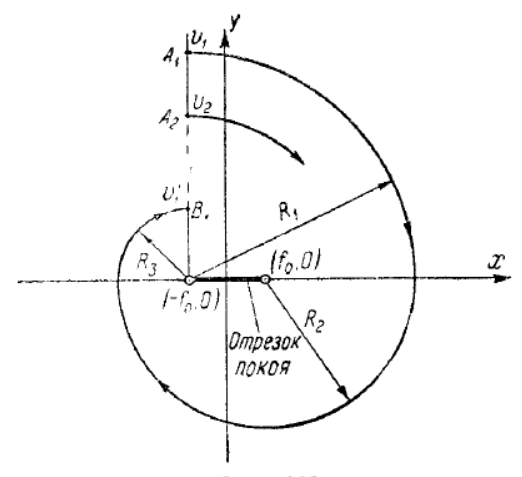
\includegraphics[width=6cm, height=6cm]{ВПВ_2}
\caption{Фазовый портрет колебаний}
\label{pic:1}
\end{figure}
\par Первая часть графика - четверть окружности радиуса $R_{1}=u_{1}$. При $R_{1} > 2f_{0}$ - движение продолжится в части графика y < 0. При $R_{1} \leqslant 2f_{0}$ - точка попадет на отрезок покоя, где попадет в положение равновесия.
\par Вторая часть графика - полуокружность радиуса $R_{2}=R_{1}-2f_{0}=u_{1}-2f_{0}$. При $R_{2} \leqslant 2f_{0}$ точка попадет на отрезок покоя, где окажется в положении равновесия. Наконец, при $R_{2} > 2f_{0}$ или $u_{1} > 4f_{0}$ точка вернется в верхнюю часть графика.
\begin{figure}[H]
\centering
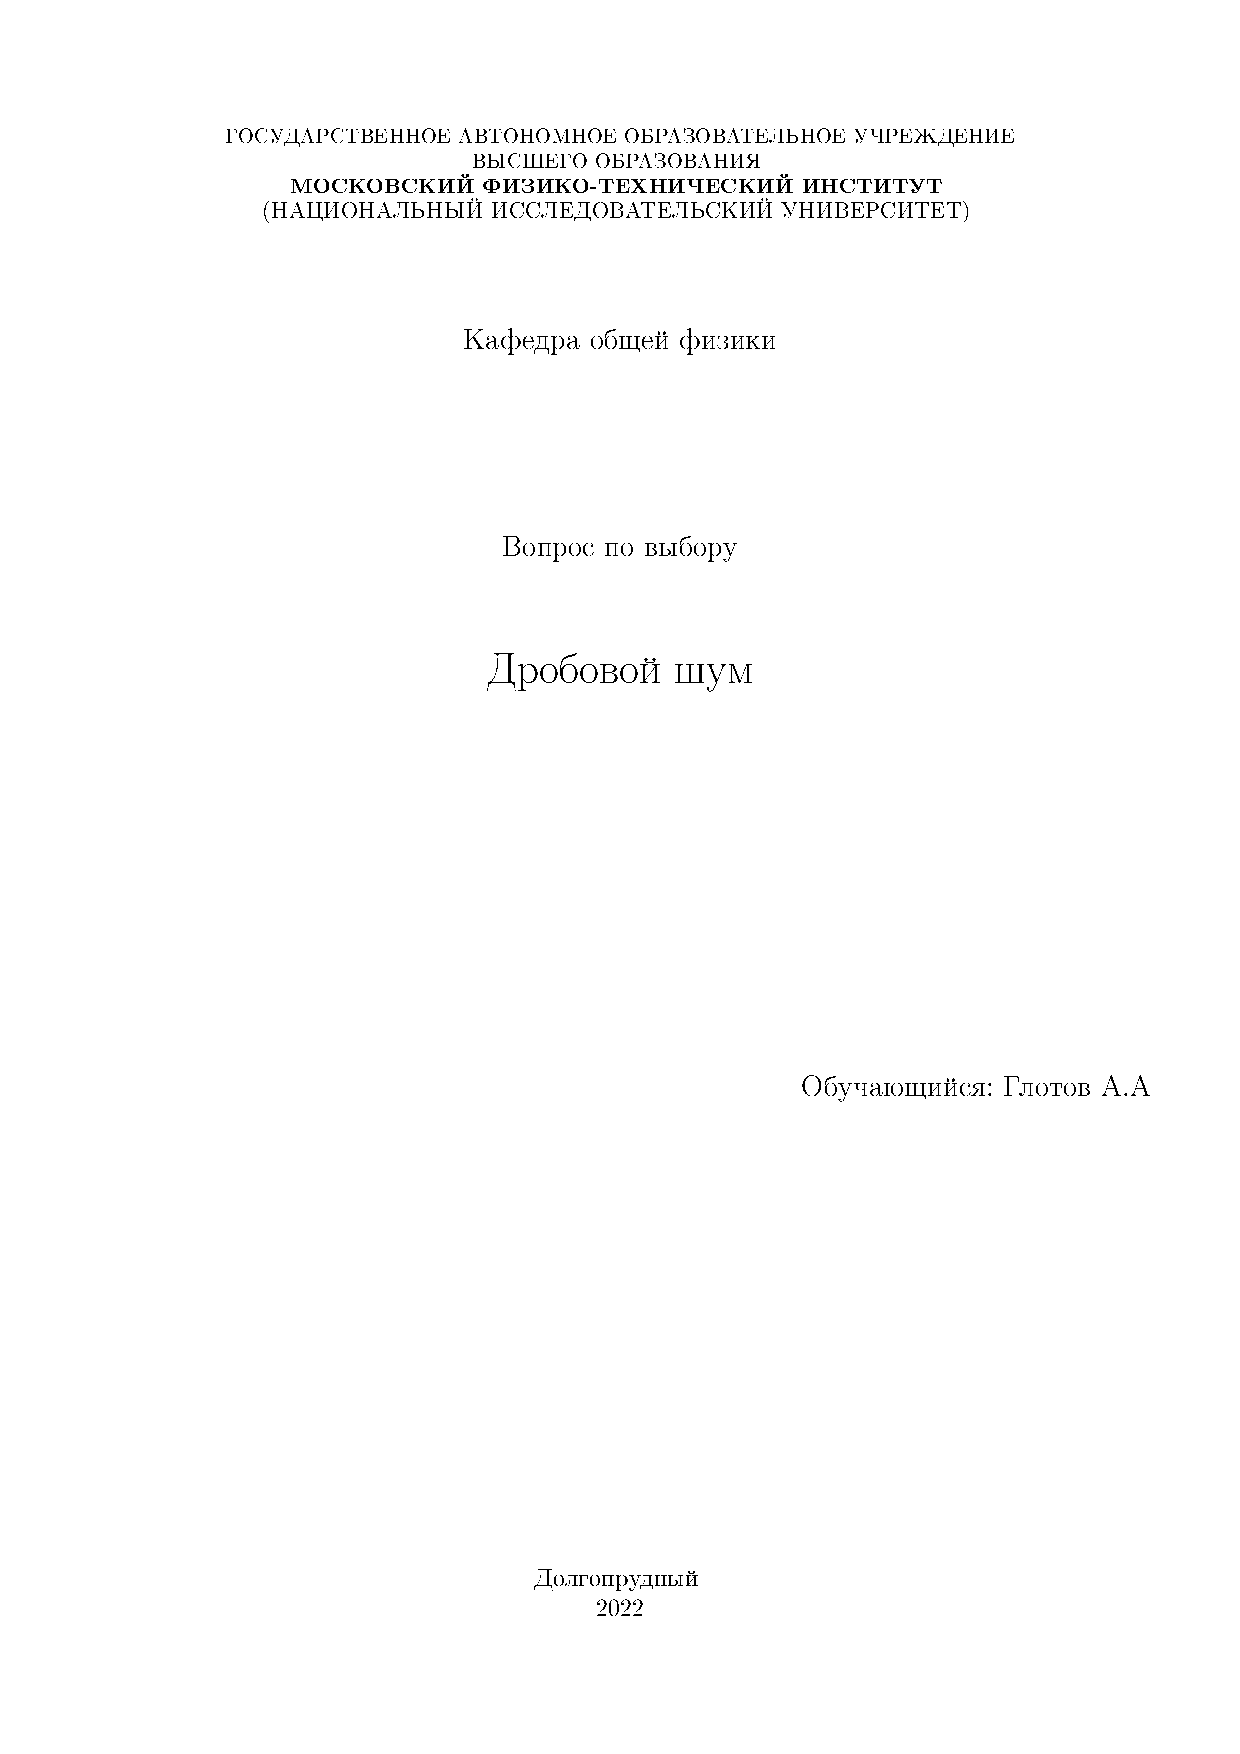
\includegraphics[width=6cm, height=6cm]{ВПВ_3}
\caption{Фазовый портрет колебаний}
\label{pic:1}
\end{figure}
\par Рассмотрим дальнейшие возможные варианты развития системы. \hfill \break
I. $a < 4f_{0}$ - колебания в системе затухают и в итоге точка окажется в положении равновесия
II. $a > 4f_{0}$ - в таком случае возможны 2 варианта.\hfill \break
$u_{1} \leqslant 4f_{0}$ Точка проходит через отрезок покоя и колебательная система оказывается в состоянии равновесия - колебания прекратились. \hfill \break
$u_{1} > 4f_{0}$ - колебания будут неограниченно нарастать \hfill \break
III. $a = 4f_{0}$ - аналогично предыдущему случаю, в зависимости от стартовых значений (причем при тех же соотношениях), колебания или затухнут при первом "проходе", или будут бесконечно поддерживаться. Однако вместо бесконечного нарастания будет поддерживаться стационарное состояние системы, зависящее от стартовых условий.
\par Данная система хоть и удовлетворяет большинству требований, однако все равно не подходит полностью - амплитуда не постоянна независимо от начальных условий \hfill \break
2.2) Примем, что $u^{2}_{1}-u^{2}_{2}=h^{2}=const$ \hfill \break
Тогда "скачок" скорости после удара зависит от "предударной" скорости маятника. В виде функции:
\begin{equation}
u^{2}_{2} = (u_{1} - 4f_{0})^{2} + h^{2}; (u_{1} > 4f_{0})
\end{equation}
Изобразим график функции 
\begin{figure}[H]
\centering
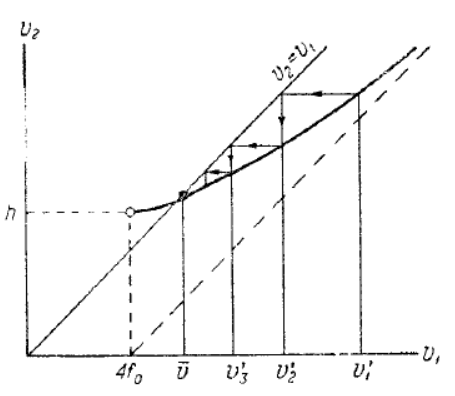
\includegraphics[width=12cm, height=9cm]{ВПВ_4}
\caption{}
\label{pic:1}
\end{figure}
\par Очевидно, что существование $u_{2}$ равносильно выполнению неравенства $h > 4f_{0}$, т.к. необходимо существование точки пересечения гиперболы и прямой. Условие $u_{1} = u_{2}$ следует из стационарности колебаний, т.е. состояние системы в двух состояниях, отличающихся во времени на целое число периодов, должно быть идентичным. Из этого же условия получаем, что:
\begin{equation}
\vec{u}^{2} = (\vec{u} - 4f_{0})^{2} + h^{2}
\end{equation}  
Откуда получаем 
\begin{equation}
\vec{u} = \frac{h^{2}}{8f_{0}} + 2f_{0}
\end{equation}
И тогда из фазовой диаграммы очевидно, что стационарная амплитуда равна
\begin{equation}
\vec{u} = \vec{u} - f_{0} = \frac{h^2}{8f_{0}} + f_{0}
\end{equation}
\end{document}

